\begin{figure}
    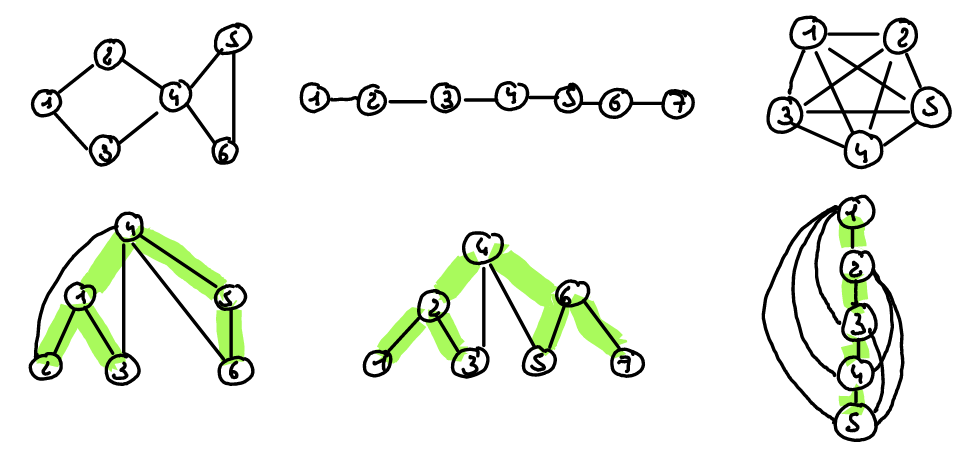
\includegraphics[width=\textwidth]{figures/treedepth-example.png}
    \caption{Examples of treedepth. (a) A graph with treedepth 3. (b) A path of size $n$ has treedepth $\lceil\log_2(n)\rceil$. (c) A clique of size $n$ has treedepth $n$. For each example, the graph is shown at the top, and the elimination forest is depicted in green at the bottom.}
    \label{fig:treedepth-example}
\end{figure}